% ===========================================================================
% Phase 3 (training): training procedure, tuning and final models.
% Owner: Muhammad Abdullah Saeed.
%
% Every result number in this file comes from report/generated/*.tex, which is written by
%     python scripts/make_training_report_assets.py
% Re-run that script after any training run instead of editing numbers by hand.
% The figure figures/training_curves_final.png is produced by the same script.
% ===========================================================================
\input{generated/training_macros}

\subsection{Training Procedure}
\label{sec:phase3_training}

\trProvisional

\paragraph{Framework and CPU rationale.}
The network is implemented in PyTorch (CPU build). It is a small multilayer perceptron
with \trParams{} trainable parameters, and the full training matrix (4{,}407{,}160 cells
$\times$ 29 features in \texttt{float32}) occupies about 0.51~GB, so the whole training set
is held in memory and mini-batches are sliced directly from tensors, without data-loader
worker processes. A GPU would add little for a network of this size, and a CPU-only setup
keeps the experiment reproducible on any team member's laptop. Training uses all but one of
the available CPU threads.

\paragraph{Data split.}
Mazes, not cells, are split 70/15/15 into train, validation and test sets (1{,}313, 281 and
282 mazes; 4{,}407{,}160, 896{,}328 and 911{,}949 labelled cells). Splitting by maze
prevents cells of one maze from appearing on both sides of the split. The assignment is
deterministic (seed 42) and stored in \texttt{results/manifests/split\_manifest.json}; the
same manifest selects the held-out test mazes for the search experiments.

\paragraph{Target and standardisation.}
The regression target is $y=h^*(n)/N$, the optimal remaining cost normalised by the grid
side $N$. Its range is $[0,\,3.18]$ rather than $[0,1]$, because an optimal path that winds
around walls can be longer than $N$ cells. The tuning compares training on the raw target
with training on the standardised target $z=(y-\mu)/\sigma$, where $\mu$ and $\sigma$ are
computed on the training split only; the selected option is \texttt{\trTargetTransform}.
The statistics stored in the final checkpoints are $\mu=\trTargetMean$ and
$\sigma=\trTargetStd$ (these are $0$ and $1$ when the raw target is selected). Predictions
are converted back to the original scale before use, and all MAE values in this report are
in units of $h^*/N$.

\paragraph{Loss.}
The network has two heads, and the training loss is
$\mathcal{L}=\mathcal{L}_{\mathrm{reg}}+\lambda\,\mathcal{L}_{\mathrm{cls}}$.
The regression term $\mathcal{L}_{\mathrm{reg}}$ is the \texttt{\trRegLoss} loss on the
(optionally standardised) target; for SmoothL1 the quadratic-to-linear transition is at
$\beta=\trSmoothBeta$. The auxiliary term $\mathcal{L}_{\mathrm{cls}}$ is the cross-entropy
over \trNumBins{} distance bins whose edges are the deciles of the training targets
(equal-frequency bins, stored in each checkpoint). The selected weight is
$\lambda=\trLambdaAux$.

\paragraph{Optimiser and regularisation.}
Parameters are updated with AdamW (learning rate \trLearningRate, weight decay
\trWeightDecay, batch size \trBatchSize), with dropout \trDropout{} between the hidden
layers. The learning rate is multiplied by \trLRFactor{} when the validation MAE has not
improved for \trLRPatience{} epochs (ReduceLROnPlateau), gradients are clipped at a norm of
\trGradClip, and training stops early after \trPatience{} epochs without improvement, with
at most \trMaxEpochs{} epochs. At each epoch the network is trained on a fresh random
subset of the training cells; the primary run uses the whole training split every epoch
and the replicate runs use 1{,}000{,}000 random cells per epoch to bound the CPU time.
The checkpoint with the lowest validation MAE is kept.

\subsection{Hyperparameter Tuning}
\label{sec:phase3_tuning}

The search space has $4\cdot2\cdot3\cdot3\cdot3\cdot3\cdot2\cdot3\cdot2=7{,}776$
combinations, far too many to train in full on a CPU, so a staged search was used. In
stage~A, 12 configurations (the default configuration plus 11 sampled at random with a
fixed seed) were trained for 5 epochs on 400{,}000 random training cells per epoch and
evaluated on a fixed subset of 100{,}000 validation cells. In stage~B, the three best
configurations were retrained for 10 epochs on 1{,}500{,}000 cells per epoch and evaluated
on the whole validation split. In stage~C, the best stage~B configuration was trained on
the full training split for up to \trMaxEpochs{} epochs with early stopping. Configurations
are ranked by validation MAE on the original $h^*/N$ scale, so that runs with different
target transforms are compared fairly. Table~\ref{tab:tuning_space} lists the tested
values and the final selection, and Table~\ref{tab:tuning_runs} lists every run.

\input{generated/tuning_space_table}

\input{generated/tuning_runs_table}

\subsection{Final Models and Training Curves}
\label{sec:phase3_final}

The selected configuration was trained with three seeds (\trSeedList). Seed~42 is the
primary model used in the main evaluation; the other seeds are replicates that indicate how
much the result depends on the random initialisation and the sampled batches. The primary
model reaches a validation MAE of \trValMAE{} (in $h^*/N$ units) at epoch \trBestEpoch{},
with a validation bin accuracy of \trValBinAcc{} and a macro-averaged F1 of \trValMacroF{}.
Over the \trNumSeeds{} seeds the validation MAE is \trMeanMAE{} $\pm$ \trStdMAE{}
(mean $\pm$ sample standard deviation); the replicates use fewer cells per epoch, so this
spread mixes the effect of the seed with that of the training budget.
Table~\ref{tab:final_training} summarises the runs and Figure~\ref{fig:training_curves}
shows the training and validation curves.

\input{generated/final_training_table}

\begin{figure}[H]
\centering
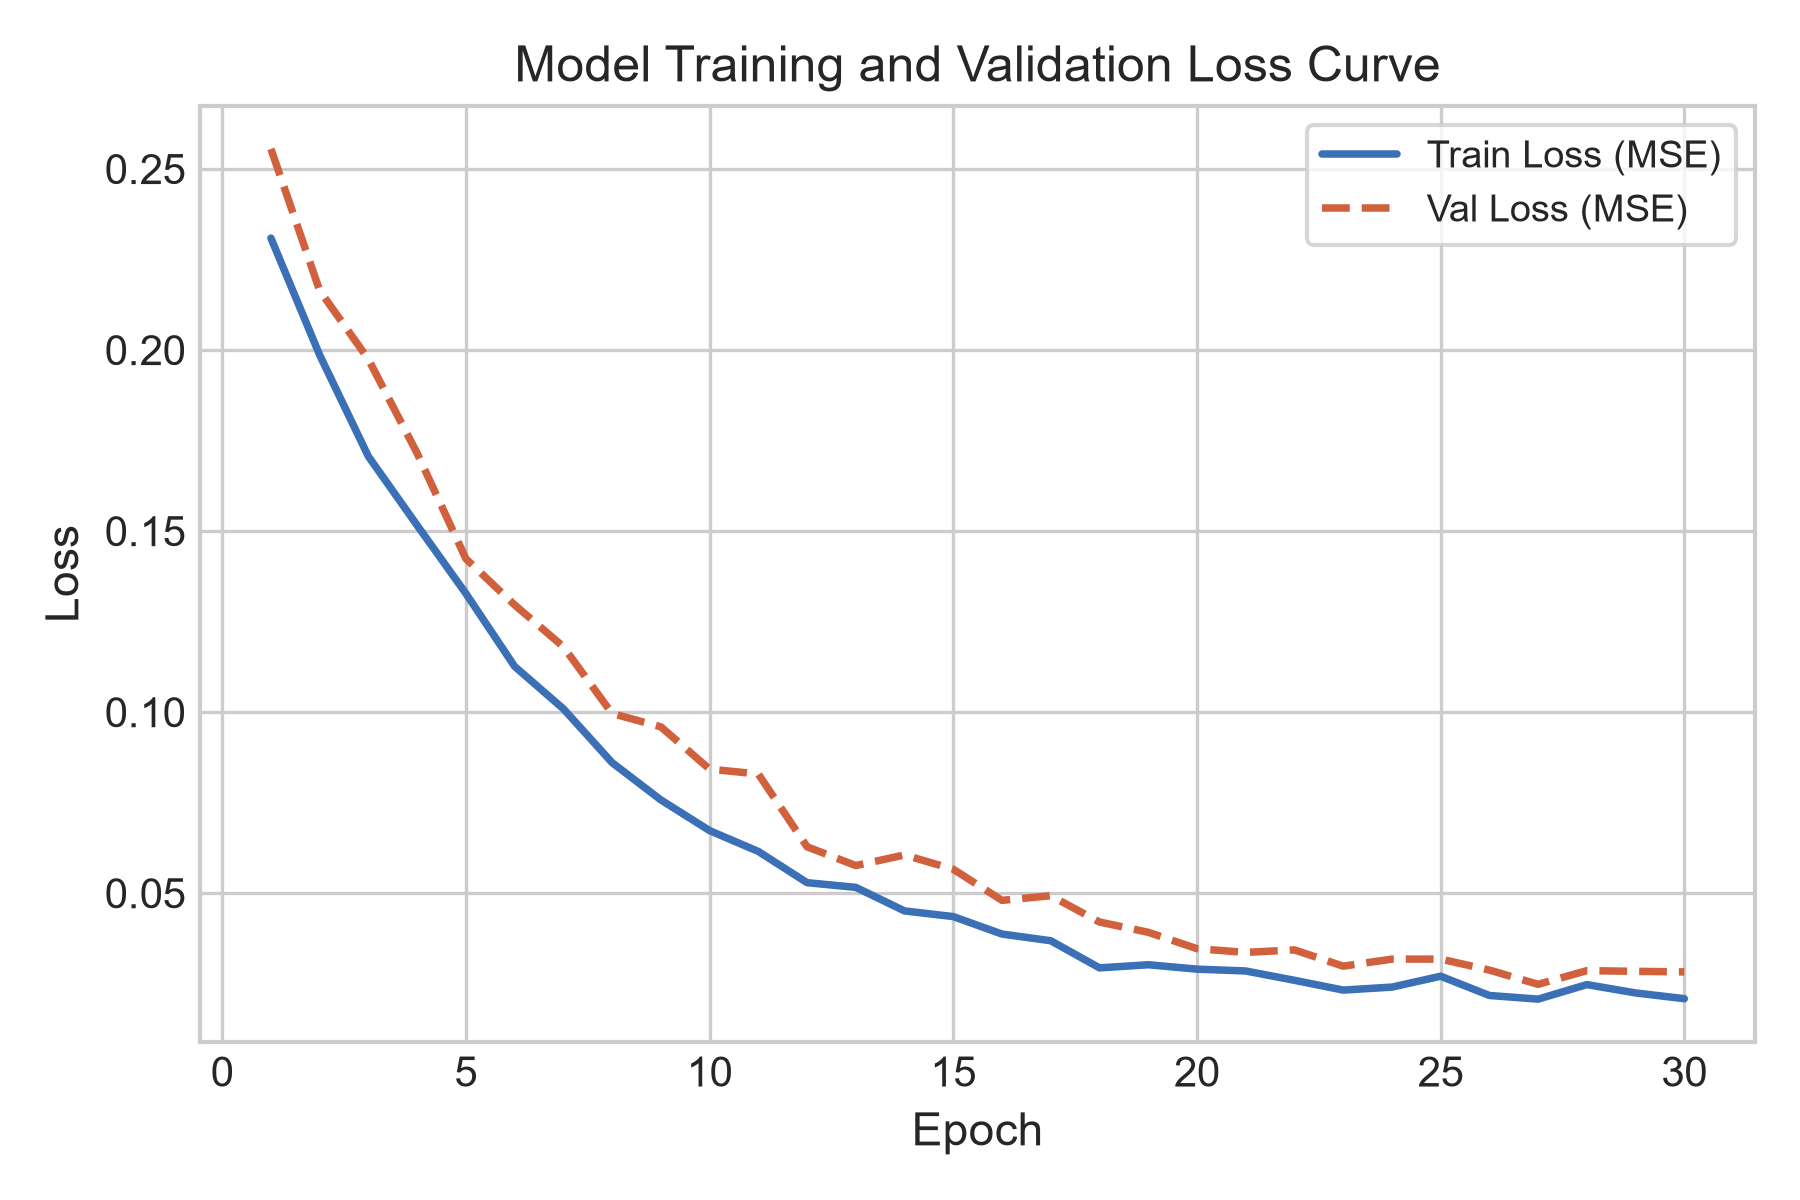
\includegraphics[width=\textwidth]{training_curves_final.png}
\caption{Training (dashed) and validation (solid) loss, validation MAE in $h^*/N$ units and
validation bin accuracy per epoch for each seed. An epoch of the primary run covers the
full training split; epochs of the replicate runs cover fewer cells.}
\label{fig:training_curves}
\end{figure}

\subsection{Reproducibility of Training}
\label{sec:phase3_repro}

All runs are controlled by a configuration file and a seed: \texttt{configs/final.yaml}
holds the selected hyperparameters, and every checkpoint stores its configuration, seed
and Git commit together with the target statistics and the bin edges. The primary model is
reproduced with
\begin{verbatim}
python -m src.train --config configs/final.yaml --seed 42 \
    --output models/neural_heuristic_seed42.pt
\end{verbatim}
On the same machine, repeating a run with the same seed reproduces the same validation MAE
up to floating-point tolerance; small numerical differences are possible across machines
with different numbers of threads. The checkpoints are hosted on Hugging Face and their
SHA256 checksums are listed in \texttt{models/README.md}.
